\documentclass{article}
\usepackage[utf8]{inputenc}
\usepackage{graphicx}
\graphicspath{ {./images/} }
\usepackage{multicol}
\usepackage[spanish, english]{babel}
\usepackage[left=3cm,right=3cm,top=3cm,bottom=3cm]{geometry}

\providecommand{\keywords}[1]{
  \small	
  \textbf{\textit{\quad \quad Keywords: }} #1}

\providecommand{\pclave}[1]{
  \small	
  \textbf{\textit{\quad \quad Palabras Clave: }} #1}

%Idiomas: \selectlanguage{english} \selectlanguage{spanish}

\begin{document}

\title{Trabajo Encargado N°2: COMPARATIVA DE TECNOLOGIAS DE DISPONIBILIDAD}
\begin{titlepage}
\begin{figure}[htb]
\begin{center}

\includegraphics[width=5cm]{logo.png}
\end{center}
\end{figure}
\vspace*{-0.25in}
\begin{center}
\large{UNIVERSIDAD PRIVADA DE TACNA}\\
\vspace*{-0.025in}
INGENIERIA DE SISTEMAS  \\

\vspace*{0.5in}
\begin{large}
TITULO:\\
\end{large}

\vspace*{0.1in}
\begin{Large}
\textbf{COMPARATIVA DE TECNOLOGIAS DE DISPONIBILIDAD} \\
\end{Large}

\vspace*{0.3in}
\begin{Large}
\textbf{CURSO:} \\
\end{Large}

\vspace*{0.1in}
\begin{large}
BASE DE DATOS 2\\
\end{large}

\vspace*{0.3in}
\begin{Large}
\textbf{DOCENTE:} \\
\end{Large}

\vspace*{0.1in}
\begin{large}
 Ing. Patrick Cuadros Quiroga\\
\end{large}

\vspace*{0.2in}
\vspace*{0.1in}
\begin{large}

Integrantes: \\
\begin{flushleft}
Briset Celia Garcia Salazar\hfill(2018062496) \\
Mathius Omar Farfan Colque\hfill(2015050991)\\
Roger Alex Aria Vela\hfill(2015050623)\\
Daniel Alejandro Gonzalez Franco\hfill(2015052599)\\
Deivis Jhonatan Flores Navarro\hfill(2018060916)\\
Luis Fernando Flores Querie\hfill(2018062394)\\

\end{flushleft}
\end{large}

\vspace*{0.1in}
\begin{large}
Tacna - Perú\\
2021
\end{large}
\end{center}
\end{titlepage}

\vspace*{\fill}
	
\begin{center}
    
\selectlanguage{spanish}
\begin{abstract}
\quad El presente artículo definira brevemente las tecnologias de alta disponibilidad. Que refiere a sistemas que estan la mayor parte del tiempo disponible, minimizando asi los periodos de inactividad. Se definira tambien los elementos que necesita un sistema de alta disponibilidad, que hace que un sistema sea altamente disponible y los componentes requeridos para esta. Además se realizo una comparativa de dos de estas tecnologias siendo estas el Sharding y el Partitioning. El sharding es la práctica de optimizar los sistemas de administración de bases de datos al separar las filas o columnas de una tabla de base de datos más grande en varias tablas más pequeñas. El Partitioning permite subdividir una tabla, un índice o una tabla organizada por índices en partes
más pequeñas.
\end{abstract}
\pclave{Alta disponibilidad, base de datos, Sharding, Partitioning, comparativa}




\selectlanguage{english}
\begin{abstract}
\quad This article briefly defines high availability technologies. Which refers to systems that are most of the time available, thus minimizing downtime. The elements that a high availability system needs, which makes a system highly available, and the components required for this, will also be defined. In addition, a comparison of two of these technologies was made, these being Sharding and Partitioning. Sharding is the practice of optimizing database management systems by separating the rows or columns of a larger database table into several smaller tables. Partitioning allows you to subdivide a table, an index or a table organized by indexes into smaller parts. 

 \end{abstract}
 
 \keywords{High Availability, database, Sharding, Partitioning, comparison} 
\end{center}
\vspace*{\fill}

\newpage 


\begin{multicols}{2}

\section{Introducción}
Hoy en dia gracias a la globalizacion los avances tecnologicos avanzan a una gran velocidad haciendo a los consumidores mas atentos y dependientes de estos servicios. Servicios como redes sociales, los repositorios virtuales e inclusive los videojuegos necesitan para su funcionamiento bases de datos  que siempre esten activos pues cuentan con clientes alrededor del mundo. Estos servicios tienen ahora la necesidad basica de siempre estar funcionando. es aqui donde entran las tecnologias de alta disponibilidad que, como su nombre lo indica, son tecnologias con el prpposito de maximizar el tiempo en el que el servicio esta activo y minimizar en los que esta inactivo.

\section{Tecnologias de disponibilidad}
En informática, el término disponibilidad se utiliza para describir el período de tiempo en que un servicio está disponible, así como el tiempo requerido por un sistema para responder a una solicitud realizada por un usuario.

La alta disponibilidad es la calidad de un sistema o componente que asegura un alto nivel de rendimiento operativo durante un período de tiempo determinado.

\begin{itemize}
\item \textbf{Disponibilidad de medición.}
La disponibilidad a menudo se expresa como un porcentaje que indica cuánto tiempo de actividad se espera de un sistema o componente en particular en un período de tiempo determinado, donde un valor del 100/100 indicaria que el sistema nunca falla.

Por ejemplo, un sistema que garantiza el 99/100 de disponibilidad en un período de un año puede tener hasta 3.65 días de tiempo de inactividad (1/100).
Estos valores se calculan en función de varios factores, incluidos los períodos de mantenimiento programados y no programados, así como el tiempo para recuperarse de una posible falla del sistema.

\end{itemize}




\textbf{¿Cómo funciona la alta disponibilidad?}

\begin{itemize}
\item La alta disponibilidad funciona como un mecanismo de respuesta a fallas para la infraestructura. La forma en que funciona es bastante simple conceptualmente, pero generalmente requiere un software y configuración especializados.
\item Al configurar sistemas de producción robustos, minimizar el tiempo de inactividad y las interrupciones del servicio a menudo es una alta prioridad.
\item Independientemente de cómo tus sistemas y software son confiables, pueden ocurrir problemas que pueden derribar tus aplicaciones o tus servidores. La implementación de alta disponibilidad de la infraestructura es una estrategia útil para reducir el impacto de este tipo de eventos.
\item Los sistemas de alta disponibilidad pueden recuperarse de la falla del servidor o componente automáticamente.
\end{itemize}

\subsection{Base de datos}

Una base de datos es particularmente importante cuando se usa un CMS como WordPress, ya que almacena la información que compone sus páginas y publicaciones.
En nuestra configuración, los nodos de la base de datos son un grupo de servidores XtraDB de Percona, la replicación sincrónica ofrece que los datos se escriben en los nodos de la base de datos secundaria al mismo tiempo que se escriben en el primario. Este método de replicación proporciona una excelente redundancia al clúster de la base de datos porque evita períodos de tiempo en los que los nodos de la base de datos no se encuentran en estados coincidentes. Galera también proporciona replicación multimaestro , lo que significa que cualquiera de los nodos de la base de datos puede responder a las consultas de los clientes.


\subsection{¿Qué hace que un sistema esté altamente disponible?}
Uno de los objetivos de alta disponibilidad es eliminar puntos únicos de fallo en tu infraestructura. Un único punto de fallo es un componente de tu pila de tecnología que causaría una interrupción del servicio si no estuviera disponible.
Como tal, cualquier componente que es un requisito para el funcionamiento correcto de la aplicación que no tiene la redundancia es considerado como un único punto de fallo.
Para eliminar puntos únicos de fallo, cada capa de yu pila debe estar preparada para la redundancia.

La capa del servidor web en este escenario no es un único punto de fallo porque:

\begin{itemize}
\item Componentes redundantes para la misma tarea están en su lugar.
\item El mecanismo en la parte superior de esta capa (el equilibrador de carga) puede detectar fallos en los componentes y adaptar su comportamiento para una recuperación oportuna.
\end{itemize}

\subsection{¿Qué componentes del sistema se requieren para alta disponibilidad?}
Hay varios componentes que deben tenerse en cuenta cuidadosamente para implementar la alta disponibilidad en la práctica.
Mucho más que una implementación de software, la alta disponibilidad depende de factores como:

\begin{itemize}
\item Medio ambiente: si todos tus servidores están ubicados en la misma área geográfica, una condición ambiental como un terremoto o una inundación podría destruir todo el sistema. Tener servidores redundantes en diferentes centros de datos y áreas geográficas aumentará la confiabilidad.
\item Hardware: los servidores de alta disponibilidad deben ser resistentes a los cortes de energía y fallos de hardware, incluidos los discos duros y las interfaces de red.
\item Software: toda la pila de software, incluido el sistema operativo y la propia aplicación, debe estar preparada para manejar fallos inesperados que podrían requerir un reinicio del sistema, por ejemplo.
\item Datos: la pérdida de datos y la inconsistencia pueden ser causadas por varios factores, y no se limita a fallos en el disco duro. Los sistemas de alta disponibilidad deben tener en cuenta la seguridad de los datos en caso de fallo.
\item Red: las interrupciones de red no planificadas representan otro posible punto de fallo para los sistemas de alta disponibilidad. Es importante que exista una estrategia de red redundante para posibles fallos.
\end{itemize}

\subsection{¿Qué software se puede usar para configurar la alta disponibilidad?}

Cada capa de un sistema altamente disponible tendrá diferentes necesidades en términos de software y configuración. Sin embargo, a nivel de aplicación, los equilibradores de carga representan una pieza esencial de software para crear cualquier configuración de alta disponibilidad.

HAProxy (proxy de alta disponibilidad) es una opción común para el equilibrio de carga, ya que puede manejar el equilibrio de carga en varias capas y para diferentes tipos de servidores, incluidos los servidores de bases de datos .

Al avanzar en la pila del sistema, es importante implementar una solución redundante confiable para el punto de entrada de su aplicación, normalmente el equilibrador de carga. Para eliminar este único punto de falla, como se mencionó anteriormente, necesitamos implementar un grupo de equilibradores de carga detrás de una IP flotante. Corosync y Pacemaker son opciones populares para crear dicha configuración, tanto en servidores Ubuntu como CentOS.


\section{Comparativa de tecnologías de disponibilidad}

\subsection{Sharding }
Sharding es la práctica de optimizar los sistemas de administración de bases de datos al separar las filas o columnas de una tabla de base de datos más grande en varias tablas más pequeñas. Las nuevas tablas se denominan "fragmentos" (o particiones), y cada nueva tabla tiene el mismo esquema pero filas únicas (como es el caso de la "fragmentación horizontal") o tiene un esquema que es un subconjunto adecuado del esquema de la tabla original. (como es el caso de la "fragmentación vertical").

\subsubsection{¿Por qué se utiliza Sharding? }

Sharding es un concepto común en arquitecturas de bases de datos escalables. Al fragmentar una tabla más grande, puede almacenar los nuevos fragmentos de datos, denominados fragmentos lógicos, en varios nodos para lograr una escalabilidad horizontal y un rendimiento mejorado. Una vez que el fragmento lógico se almacena en otro nodo, se denomina fragmento físico.

Al ejecutar una base de datos en una sola máquina, eventualmente alcanzará el límite de la cantidad de recursos informáticos que puede aplicar a cualquier consulta y, obviamente, alcanzará una cantidad máxima de datos con los que puede trabajar de manera eficiente. Al escalar horizontalmente, puede habilitar un diseño de base de datos flexible que aumenta el rendimiento de dos maneras clave:

\begin{itemize}
    \item Con el procesamiento masivamente paralelo, puede aprovechar todos los recursos informáticos de su clúster para cada consulta.
    \item Debido a que los fragmentos individuales son más pequeños que la tabla lógica en su conjunto, cada máquina tiene que escanear menos filas al responder a una consulta.
\end{itemize}

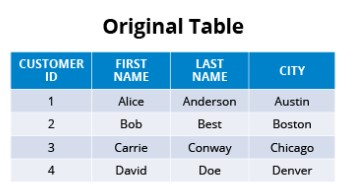
\includegraphics[width=6cm]{images/originaltable.jpg}

\textbf{Horizontal sharding }

Es eficaz cuando las consultas tienden a devolver un subconjunto de filas que a menudo se agrupan. Por ejemplo, las consultas que filtran datos basados en rangos de fechas cortos son ideales para la fragmentación horizontal, ya que el rango de fechas necesariamente limitará las consultas a solo un subconjunto de los servidores.

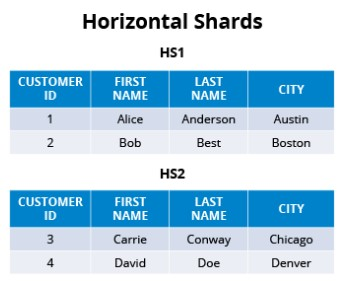
\includegraphics[width=6cm]{images/horizontal.jpg}

\textbf{Vertical sharding }

Es eficaz cuando las consultas tienden a devolver solo un subconjunto de columnas de los datos. Por ejemplo, si algunas consultas solo solicitan nombres y otras solo direcciones, los nombres y direcciones se pueden dividir en servidores separados.

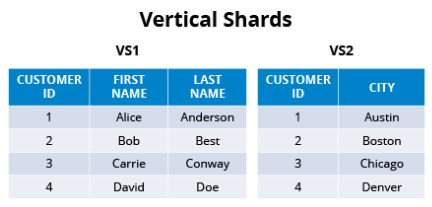
\includegraphics[width=6cm]{images/vertical.jpg}


\subsection{Partitioning}
El particionamiento permite subdividir una tabla, un índice o una tabla organizada por índices en partes
más pequeñas. Cada parte del objeto de base de datos se denomina partición. Cada partición tiene su
propio nombre, y puede, opcionalmente, tener sus propias características de almacenamiento. Desde la
perspectiva de un administrador de base de datos, un objeto particionado tiene múltiples partes que
pueden administrarse ya sea de manera conjunta o individual. Esto da al administrador una flexibilidad
considerable en la administración del objeto particionado. No obstante, desde la perspectiva de la
aplicación, una tabla particionada es idéntica a una tabla no particionada; no se necesitan modificaciones
cuando se accede a una tabla particionada utilizando comandos SQL DML.

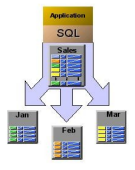
\includegraphics[width=6cm]{images/partitioning.png}

\subsection{Beneficios del partitioning}
El particionamiento puede brindar grandes beneficios a una amplia variedad de aplicaciones al mejorar
la capacidad de administración, el desempeño y la disponibilidad. No es inusual que el particionamiento
mejore mucho más el desempeño de ciertas operaciones de mantenimiento y consultas. Además, el
particionamiento puede reducir enormemente el costo total de propiedad de los datos, al utilizar un
enfoque de “archivo por niveles” para mantener la información relevante más antigua aún online en
dispositivos de almacenamiento de bajo .
También permite a los diseñadores y administradores de base de datos abordar
algunos de los problemas más difíciles planteados por las aplicaciones de vanguardia. Es una
herramienta clave para crear sistemas de múltiples terabytes o sistemas con requisitos de disponibilidad
extremadamente altos.

\subsection{Estrategias basicas de Partitioning}
Métodos de distribución de datos fundamentales que regulan cómo se
ubicarán los datos en las distintas particiones individuales, a saber:
\begin{itemize}
    \item Rango: Los datos se distribuyen de acuerdo con el rango de valores de la clave de
          particionamiento (para una columna de fechas como clave de partición, la partición 'January7
          2007' contiene filas con los valores de clave de partición entre '01-JAN-2007' y '31-JAN-2007').
          La distribución de datos es continua, sin baches y el límite más bajo del rango se define
          automáticamente por el límite más alto del rango precedente.
    \item Lista: La distribución de datos se define por un listado de valores de la clave de partición (para
          una columna de regiones como clave de partición, la partición 'North America' puede contener
          valores como 'Canada', 'USA', y 'Mexico'). Una partición especial 'DEFAULT' puede ser
          definida para reunir todos los valores de una clave de partición que no se encuentren
          explícitamente definidos en ninguna de las listas. 
    \item Elección Arbitraria: Un algoritmo de elección arbitraria se aplica a la clave de partición para
          determinar la partición para una fila determinada. A diferencia de los otros dos métodos de
          distribución de datos, la elección arbitraria no brinda ningún mapeo lógico entre los datos y una
          partición. 
\end{itemize}
Utilizando los métodos de distribución de datos antes mencionados, una tabla puede particionarse ya sea
como una única tabla o una tabla particionada compuesta:
\begin{itemize}
    \item Particionamiento Único (un solo nivel): Una tabla se define al especificar una de las
          metodologías de distribución de datos, utilizando una o más columnas como clave de partición.
          Usted puede especificar las tablas particionadas por Rango, Lista y Elección Arbitraria. 
          
   \item Particionamiento Compuesto: Para definir una tabla particionada compuesta se utiliza una
         combinación de dos métodos de distribución de datos. Primero, la tabla se particiona con un
         primer método de distribución de datos y luego cada partición se vuelve a dividir en
         subparticiones utilizando un segundo método de distribución de datos. Todas las subparticiones
         para una partición determinada en conjunto representan un subgrupo lógico de datos. Por
         ejemplo, una tabla compuesta particionada por rango-elección arbitraria primero se particiona
         por rango y después cada partición por rango se subparticiona utilizando la técnica de partición
         por elección arbitraria.
        Las técnicas de partición compuesta disponibles son: rango-elección arbitraria, rango-lista,
        rango-rango, lista-rango, lista-lista, y lista-elección arbitraria. 
    \item Las tablas organizadas por índices (IOTs) pueden particionarse utilizando el particionamiento
        por rango, elección arbitraria y lista. El particionamiento compuesto no está respaldado por las
        IOT.
\end{itemize}

\subsection{ Comparativa entre Sharding y Partitioning }

Sharding y Partitioning se tratan de dividir un gran conjunto de datos en subconjuntos más pequeños. La diferencia es que la fragmentación (sharding) implica que los datos se distribuyen en varias computadoras, mientras que la partición no. El particionamiento consiste en agrupar subconjuntos de datos dentro de una sola instancia de base de datos. En muchos casos, los términos fragmentación y partición se utilizan incluso como sinónimos, especialmente cuando van precedidos de los términos "horizontal" y "vertical". Por lo tanto, "fragmentación horizontal" y "partición horizontal" pueden significar lo mismo.




\section{Conclusiones}
\begin{itemize}
    \item   Sharding y Partitioning se tratan de dividir un gran conjunto de datos en subconjuntos más pequeño.
    Estas particiones se denominan, por tanto, shardss.(Fragmentos)
    
    \item El sharding se emplea en la arquitectura de bases de datos porque puede mejorar el rendimiento de una base de datos o de un motor de búsqueda.
    
    \item sharding nos ofrece unos accesos de gran veloidad,basicamente se ocupa de que se reduzca el volumen de latencia y el rendimiento sea superior.
    
    \item Partitioning permite descomponer tablas e índices muy grandes en partes más pequeñas y manejables que se denomina particiones . Cada partición es un objeto independiente con su propio nombre y, opcionalmente, sus propias características de almacenamiento.    
    
    \item Partitioning puede mejorar la disponibilidad de aplicaciones asegurándose de que todo el conjunto de datos no constituye un punto de error único y que subconjuntos individuales del conjunto de datos pueden administrarse de forma independiente.

    \item La fragmentación(sharding) de bases de datos puede ser una gran solución para los clientes que buscan escalar su base de datos horizontal y verticalmente. Sin embargo, también agrega complejidad y un punto de falla a la aplicación. La fragmentación puede ser importante para algunos, pero el tiempo y los recursos para crear y mantener la arquitectura podrían superar los beneficios para otros.
 
    
\end{itemize}
 

\section{Recomendaciones}
\begin{itemize}
    \item  Antes de aplicar una de estas tecnologias se debe de identificar bien la cantidad de datos con el que se trabaja y otras necesidades que se tengan.
    
     \item  se recomienda que antes de usar cualquier tecnologia disponible se analize hacia donde va dirigido, cuales son los limites, que magnitud tendra y evitar complejidad.
    
\end{itemize}
\end{multicols}
\newpage

\begin{thebibliography}{XXX00000}

    \bibitem{1}Database Concepts.(2021, 20 septiembre). Oracle Help Center. https://docs.oracle.com/en/database/oracle/oracle-database/19/cncpt/partitions-views-and-other-schema-objects.html#GUID-91498562-1809-4E67-B7AD-9718ED60DEFFw3
    
    \bibitem{2} Partitioning. (s. f.). InfoSphere Information Server. Recuperado 20 de septiembre de 2021, de https://www.ibm.com/docs/en/iis/11.3?topic=data-partitioning

    \bibitem {3}Academy, B. (2020, 1 junio). ¿Qué es Sharding? Bit2Me Academy. https://academy.bit2me.com/que-es-sharding/
  
    
    \bibitem{4} ¿Qué es el sharding en MongoDB? ¿Cómo funciona el sharding en MongoDB? | ramoncarrasco.es. (s. f.). ramoncarrasco.es. Recuperado 20 de septiembre de 2021, de https://www.ramoncarrasco.es/es/content/es/kb/141/que-es-el-sharding-en-mongodb-como-funciona-el-sharding-en-mongodb
  
    
 
    \bibitem{5} Sharding — MongoDB Manual. (s. f.). Mongo Db - Documentation. Recuperado 02 de septiembre de 2020, de https://docs.mongodb.com/manual/sharding/


    \bibitem{6} Yves Duquesnoy, P. (s. f.). Escalabilidad y Sharding. InterSystems Corporation. Recuperado 15 de febrero de 2018, de https://www.intersystems.com/es/wp-content/uploads/sites/10/Escalabilidad_y_Sharding.pdf
    
    \bibitem{7}  Sarangam, A.(2021 31 Marzo) Database Sharding: A Simple Overview In 2021. recuperado de https://www.jigsawacademy.com/blogs/cloud-computing/database-sharding

    
    \bibitem{8} hazelcast. (s. f.). What Is Sharding?. recuperado de https://hazelcast.com/glossary/sharding/
    
 \end{thebibliography}
    
    


\end{document}
